\section{Project Overview}

\subsection{Introduction}

\subsubsection{Background}

The first satellite, Sputnik 1, was launched by the Soviet Union on October 4, 1957. This event marked the start of the space race, leading to new technological, scientific, and political developments \cite{nasa-sputnik}. Since then, 23030 satellites have been launched \cite{esa-debris}. Satellites orbiting Earth can be split into 3 catagories:

\begin{itemize}
    \item \ac{LEO} : 160 km - 2,000 km

    \item \ac{MEO} : 2,000 km - 35,786 km

    \item \ac{GEO} : 35,786 km
\end{itemize}

For decades interest lied in \ac{GEO} satellites, with Syncom becoming the first \ac{GEO} satellite in 1963~\cite{nasa-syncom}. Being in geosynchronous orbit meant that satellites could stay at a specific position above Earth, allowing for constant communication with a specific area on Earth. This made these satellites ideal for communication and weather monitoring. However, \ac{GEO} satellites have high latency due to their distance from Earth, making them less suitable for real-time applications.

Since then the most significant change in satellite technology has been the development of \ac{LEO} satellites. Although they were first developed in the 1990s, these satellites have only really become widely used in the last decade. Companies like OneWeb and Starlink have launched constellations of \ac{LEO} satellites to provide low-latency internet access across the globe~\cite{reliasat-evolution}. These developments denoted a transition in the commercial communication satellite business from small numbers of large geostationary satellites towards constellations of hundreds of smaller lower satellites in low earth orbit.

Fueled by this new idea, the global space industry accelerates as the number of satellites launched annually continues to rise. Both governments and private entities are allocating significant resources to satellite research and development for applications such as communication, navigation, Earth observation, atmospheric characterization, and military purposes.

\subsubsection{Project Motivation}

With the increasing complexity of mission requirements, the need for more advanced satellite technologies has increased. Specifically, the need for efficient and reliable propulsion systems has become crucial for satellite operations. Satellites require propulsion for various reasons, including orbit insertion, station-keeping, attitude control, deorbiting at the end of their operational life, and formation flying. Additionally, as spent rockets, satellites and other space trash accumulate in orbit, the likelihood of collisions with debris has increased. Unfortunately, collisions create more debris creating a runaway chain reaction of collisions and more debris known as the Kessler Syndrome~\cite{nasa-kessler}.

There are two main types of propulsion systems used in satellites: chemical propulsion and \ac{EP}. Satellites have traditionally used chemical propulsion systems, although there is now a huge shift towards \ac{EP} systems with Space X's Starlink constellation being the largest adopter of EP technology.

Chemical propulsion uses a fuel and an oxidizer, converting energy stored in the chemical bonds of the propellants, to produce a short, powerful thrust, or what we see as fire. It’s loud and exciting, but not all that efficient. Chemical propulsion is said to be "energy limited" because the chemical reactants have a fixed amount of energy per unit mass, which limits the achievable exhaust velocity or \ac{$I_{sp}$}.

Electric propulsion systems use energy collected by either solar arrays or a nuclear reactor to generate thrust by using electric, and possibly magnetic, processes to ionize and accelerate a propellant. It is a technology aimed at achieving thrust with high-exhaust velocities, which results in a reduction in the amount of onboard propellant required for a given space mission or space-propulsion application compared to other conventional propulsion methods. Reduced propellant mass can significantly decrease the launch mass of a spacecraft or satellite, leading to lower costs from the use of smaller launch vehicles to deliver a desired mass into orbit or to a deep space target. \cite{fundamentals-of-electric-propulsion}
It can reduce the amount of fuel, or propellant, needed by up to 90\% compared to chemical propulsion systems, saving millions in launch costs while providing greater mission flexibility. \cite{nasa-electrifying-propulsion}

\begin{figure}[H]
    \centering
    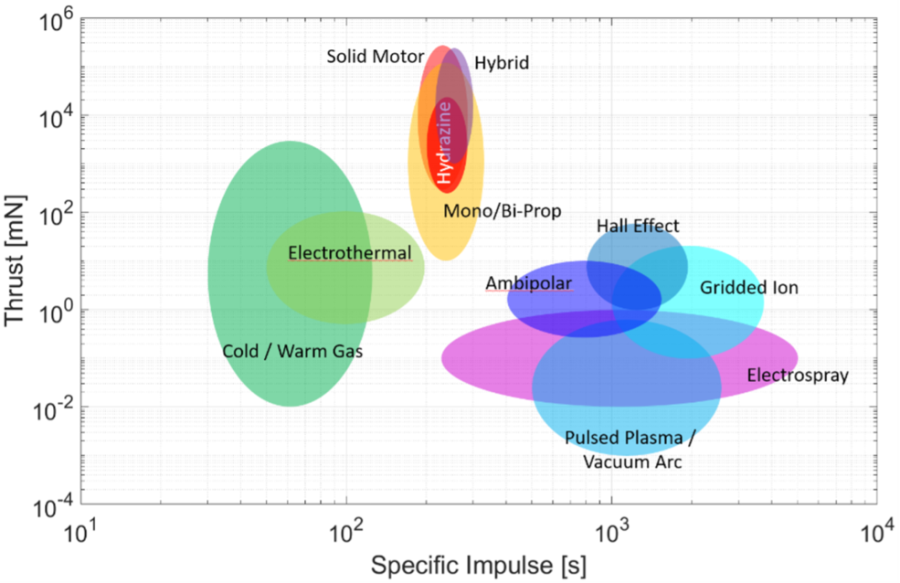
\includegraphics[width=0.9\textwidth]{images/Concepts/thrust vs specific impulse for electric systems.png}
    \captionsetup{justification=centering}
    \caption{Typical small spacecraft in-space propulsion (thrust vs specific impulse) \\ Chemical Thrusters shown in shades of red and Electric Thrusters shown in shades of blue\cite{nasa-inspace-propulsion}.}
    \label{fig:thrust_vs_specific_impulse_propulsion_systems}
\end{figure}

\subsubsection{Relevance}

As the technology matures and becomes more widely adopted, we can see an increasing interest in the space and satellite industry by the goverment of Canada. The \ac{CSA} has been actively encouraging development in the industry through initiatives such as the "Call for Ideas - Science and technology small payloads for space missions"~\cite{csa-call-for-ideas}. The \ac{CSA} also initated a "Consultation on Changes to Licensing Requirements and Conditions of Licence on Space Debris Mitigation" \cite{csa-space-debris-mitigation}, which aims to address the growing concern of space debris. It proposes mandating active propulsion systems, with redundancy, for all Non-Geostationary Satellite Orbit (NGSO) satellites operating at or above 400 kilometers. This can severley increase the system and integration complexity for small satellites. Hence, now more than ever, there is a need to develop modern, efficient, and reliable propulsion systems for satellites. This shows that the goverment of Canada is aware of the increasing importance of the space industry and is taking steps to ensure its growth and sustainability.

